\documentclass{article}
\usepackage[utf8]{inputenc}
\usepackage[a4paper, top=1in, bottom=1in, left=1in, right=1in]{geometry} 
\usepackage{graphicx}
\setlength\parindent{0pt} % Removes all indentation from paragraphs - comment this line for an assignment with lots of text

\usepackage{algorithm}
\usepackage[noend]{algpseudocode}

\usepackage{amsmath}
\usepackage{amssymb}
\usepackage{tikz}
\usepackage{pgfplots}

\newcommand\tab[1][1cm]{\hspace*{#1}}
\newcommand{\vect}[1]{\boldsymbol{#1}}

\title{\huge{\textbf{Data Mining Note}}}
\author{Chauncey Liu}
\date{\today}

\begin{document}
 
\maketitle
 
\tableofcontents

\newpage
 
\section{Association Rules and Frequent Pattern Mining}
\subsection{The Frequent Pattern Mining Model}
\textbf{Basic Concepts:}
\begin{itemize}
\item Items $I = \{i_1, i_2, ..., i_m\}$, a set of literals 
\item Itemset $X$ (transaction): set of items $X \subseteq I$
\item Database $D$: set of transactions $T_i$ where $T_i \subseteq I$
\item $T$ contains $X$: $X \subseteq T$
\item Items in transactions or itemsets are sorted in lexicographic order
\item Length of itemset: number of elements of itemset
\item k-itemset: itemset of length $k$
\end{itemize}

\textbf{Supermarket example:}
\begin{itemize}
  \item Items $I = \{Bread, Butter, Milk, Eggs, Yogurt\}$ 
  \item Itemset $X$, Transaction $T$: 
    \begin{itemize}
      \item $X_1 = \{Bread, Butter\}$, $X_2 = \{Eggs, Milk\}$
      \item $T_1 = \{Bread, Butter, Milk\}$, $T_2 = \{Eggs, Milk, Yogurt\}$
    \end{itemize}
  \item Database $D$: set of transactions $T_i$ where $T_i \subseteq I$
    \begin{itemize}
      \item $T_1 = \{Bread, Butter, Milk\}$, $T_2 = \{Eggs, Milk, Yogurt\}$
      \item $D = \{T_1, T_2\} = \{\{Bread, Butter, Milk\}, \{Eggs, Milk, Yogurt\}\}$
    \end{itemize}
  \item $T$ contains $X$: $X \subseteq T$
    \begin{itemize}
      \item $X_1 = \{Bread, Butter\}$, $T_1 = \{Bread, Butter, Milk\}$
      \item $X_1 \subseteq T_1$
    \end{itemize}
  \item Items in transactions or itemsets are sorted in lexicographic order
  \item Length of itemset: number of elements of itemset
  \item k-itemset: itemset of length $k$
\end{itemize}

\textbf{Further Concept}
\begin{itemize}
  \item Support of itemset $X$ in $D$: percentage of transactions in $D$ containing $X$
    \begin{itemize}
      \item $sup(X, D) = \frac{|{T \in D | X \subseteq T}|}{|D|}$
    \end{itemize}
  \item Frequent itemset $X$ in $D$: item set X with
    \begin{itemize}
      \item $freq(X, D) :\Leftrightarrow sup(X, D) \ge minsup$
    \end{itemize}
  \item Association rule: implication of the form $ X \Rightarrow Y$
    \begin{itemize}
      \item where $X \subseteq I, Y \subseteq I$ and $X \cap Y = \varnothing$
    \end{itemize}
  \item Support $s$ of association rule $X \Rightarrow Y$ in $D$:
    \begin{itemize}
      \item indicates how frequently the itemset appears in the dataset
      \item support of $X \cup Y$ in $D$
      \item $s = \frac{|{T \in D | (X \cup Y) \subseteq T}|}{|D|}$
    \end{itemize}
  \item Confidence $c$ of association rule $X \Rightarrow Y$ in $D$:
    \begin{itemize}
      \item indicates how often the rule has been found to be true
      \item percentage of transactions containing $Y$ in the subset of all transactions in $D$ that contain $X$
      \item $c = \frac{|{T \in D | (X \cup Y) \subseteq T}|}{|{T \in D | X \subseteq T}|} = \frac{\sup(X \cup Y)}{\sup(X)}$
    \end{itemize}
\end{itemize}

\newpage

\subsection{Association Rules}
\subsubsection{Mining Association Rules}
1. Determine the frequent itemsets in the database \\
Naive algorithm: count the frequencies of all k-itemsets $\subseteq I$, inefficient since $\binom mk$ such itemsets \\

2. Generate the association rules from the frequent itemsets \\
Itemset $X$ frequent and $A \subseteq X$ \\
$A \Rightarrow (X-A)$ satisfies minimum support constraint (confidence remaining to be checked)

\subsubsection{Itemset Lattice}
\begin{itemize}
  \item Lattice: a partially ordered set with unique least upper bound and greatest lower bound.
  \item Itemset lattice:
    \begin{itemize}
      \item elements: itemsets $X_1 \subseteq I, X_2 \subseteq I, ..., X_n \subseteq I$
      \item partial order: $X_1 < X_2 :\Leftrightarrow X_1 \subset X_2$
      \item least upper bound: $I$
      \item greatest lower bound: $\varnothing$
    \end{itemize}
\end{itemize}

\begin{figure}[h]
\centering
\caption{Itemset Lattice}
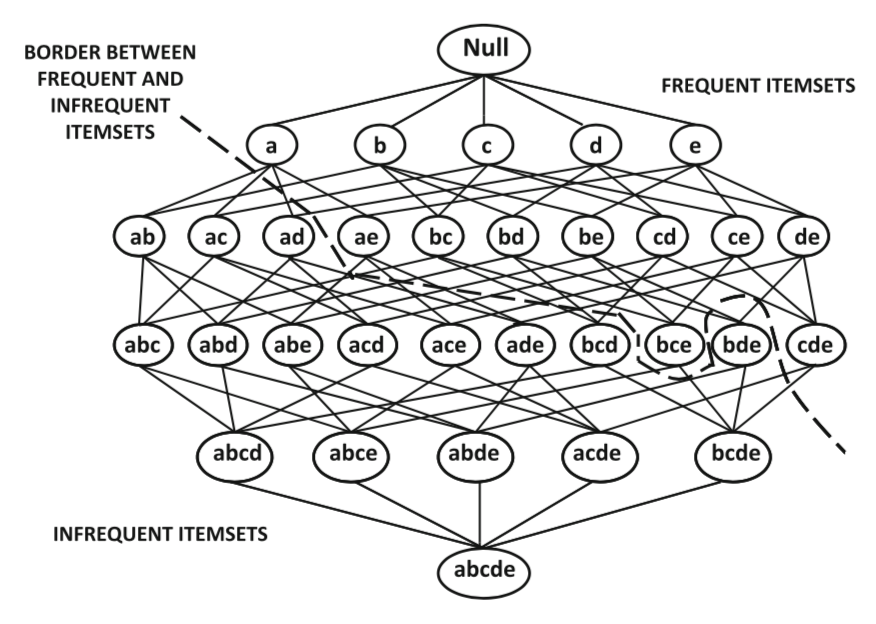
\includegraphics[width=7.5cm]{img/pic4-1.png}
\end{figure}

\subsubsection{Anti-monotonicity (downward closure) property}
Each subset of a frequent itemset is also frequent. \\
$\forall T_1 \subseteq I, T_2 \subseteq I: T_1 \subseteq T_2 \land freq(T_2, D) \Rightarrow freq(T_1, D)$ \\
because of \\
$\forall T_1 \subseteq I, T_2 \subseteq I: T_1 \subseteq T_2 \Rightarrow sup(T_1, D) \ge sup(T_2, D)$ \\

If one subset is not frequent, then superset cannot be frequent. \\
This property makes frequent itemset mining efficient, since in practice most itemsets are infrequent. 

\subsubsection{Computing the Association Rules}
\begin{itemize}
  \item Given a frequent itemset $X$
  \item For each subset $A$ of $X$, form the rule $A \Rightarrow (X - A)$
  \item Compute confidence of the rule $A \Rightarrow (X - A)$
    \begin{itemize}
      \item $confidence(A \Rightarrow (X - A)) = \frac{sup(X)}{sup(A)}$ 
    \end{itemize}
  \item Discard rules that do not have minimum confidence
  \item Store frequent itemsets with their supports in a hash table
    \begin{itemize}
      \item no DB acesses, no disk I/O
    \end{itemize}
\end{itemize}

\subsubsection{Interestingness of Association Rules}
\begin{itemize}
  \item Filter out misleading association rules
  \item Expected support for the rule $A \Rightarrow B$
    \begin{itemize}
      \item $P(A \cup B) = P(A) \cdot P(B)$
      \item assuming the idependence of A and B
    \end{itemize}
  \item Interestingness measure for rule $A \Rightarrow B$
    \begin{itemize}
      \item $\frac{P(A \cup B)}{P(A)} - P(B)$
      \item The larger this measure, the more interesting the discovered association between A and B
    \end{itemize}
  \item An alternative interestingness measure is the lift of an association rule
  \item If A and B are independent, then $P(A \cup B) = P(A) \cdot P(B)$
    \begin{itemize}
      \item i.e. $\frac{P(A \cup B)}{P(A) \cdot P(B)} = 1$
    \end{itemize}
  \item We define the lift of a rule $A \Rightarrow B$ as follows:
    \begin{itemize}
      \item $lift(A \Rightarrow B) = \frac{P(A \cup B)}{P(A) \cdot P(B)}$
      \item Can also be formulated as:
      \begin{itemize}
        \item $lift(A \Rightarrow B) = \frac{P(A \cup B) / P(A)}{P(B)} = \frac{support_{actual}}{support_{expected}}$
        \item as the ratio of the conditional probability $P(B|A)$ and the unconditional probability $P(B)$
      \end{itemize}
      \item A lift $>>1$ indicates that the discovered association between A and B is interesting.
    \end{itemize}  
\end{itemize}

\subsection{The Apriori Algorithm}
\subsubsection{Approach}
\begin{itemize}
  \item Determine first the frequent 1-itemsets, then frequent 2-itemsets, ...
  \item To determine the frequent k+1-items, consider only the k+1-items for which all k-subsets are frequent
  \item Calculation of support: one database scan counting the support for all relevant itemsets
\end{itemize}

\begin{algorithm}
\caption{Algorithm Apriori}
\begin{algorithmic}[0]
\State /* $C_k:$ set of candidate itemsets of length k */
\State /* $F_k:$ set of all frequent itemsets of length k */ \\
\Function{Apriori}{D, minsup}
\While{$F_k \ne \varnothing$}
  \State Generate $C_{k+1}$ by joining itemset-pairs in $F_k$;
  \State Prune itemsets from $C_{k+1}$ that violate anti-monotonicity;
  \State Determine $F_{k+1}$ by counting supoort of $C_{k+1}$ in D and retaining itemsets fron $C_{k+1}$ with support at least minsup;
  \State k = k + 1;
\EndWhile
\Return $\cup_k F_k$;
\EndFunction
\end{algorithmic}
\end{algorithm}

\newpage

\subsubsection{Candidate Generation}
Requirements for set $C_k$ of candidate itemsets
\begin{itemize}
  \item Superset of $F_k$
  \item Significantly smaller than set of all k-subsets of $I$
\end{itemize}

Step1: Join
\begin{itemize}
  \item Frequent k-1-itemsets $p$ and $q$, p and q are joined if they aggre in their first $k-2$ items
  \item E.g. $p \in F_{k-1} = \{1,2,3\}$, $q \in F_{k-1} = \{1,2,4\} \Rightarrow (1,2,3,4) \in C_k$
  \item Choose first k-2 items to avoid duplication without missing any candidates
\end{itemize}

Step2: Pruning
\begin{itemize}
  \item Remove all elements from $C_k$ having a k-1-subset not contained in $F_{k-1}$
  \item E.g. $F_3 = \{(1,2,3), (1,2,4), (1,3,4), (1,3,5), (2,3,4)\}$
  \item After join step: $C_4 = \{(1,2,3,4), (1,3,4,5)\}$
  \item In pruning step: remove $(1,3,4,5)$ since subsets $(1,4,5), (3,4,5)$ are missing
  \item $C_4 = \{(1,2,3,4)\}$
\end{itemize}

\subsubsection{Support Counting}
\textbf{for each} candidate $c \in c_k$ \textbf{do} c.count = 0; \\
\textbf{for each} transaction $T \in D$ \textbf{do} \\
\tab $CT := subset(C_k, T);$ // all candidates from $C_k$ that are contained in transaction $T$ \\
\tab \textbf{for each} candidate $c \in CT$ \textbf{do} c.count++; \\
$F_k := \{c \in C_k | (c.count / |D|) \ge minsup\}$\\

To achieve one scan over the database D, $subset(C_k, T)$ should be implemented properly. Thus we need Hash Tree.

\subsubsection{Hash Tree}
Hash tree as a data stucture for $C_k$
\begin{itemize}
  \item Leaf node: records list of itemsets (with frequencies)
  \item Inner node: contains hash table (apply hash function to d-th elements), each hash bucket at level $d$ references son node at level $d+1$
  \item Root has level 1
\end{itemize}

Finding an itemset
\begin{itemize}
  \item Start from the root
  \item At level $d$: apply hash function $h$ to the d-th element of the itemset.
\end{itemize}

Inserting an itemset 
\begin{itemize}
  \item Find the corrsponding leaf node and insert new itemset
  \item In case of overflow:
  \begin{itemize}
    \item Covert leaf node into inner node and create all its son nodes (new leaves).
    \item Distribute all entries over the new leaf nodes according to hash function $h$.
  \end{itemize}
\end{itemize}

\newpage

Find all candidates contained in $T = (t_1 t_2 t_3 ... t_m)$
\begin{itemize}
  \item At root
  \begin{itemize}
    \item Determine hash values $h(t_i)$ for each item $t_i$ in $T$
    \item Continue search in all correspoding son nodes
  \end{itemize}

  \item At inner node of level $d$
  \begin{itemize}
    \item Assumption: innder node has been reached by hashing $t_i$
    \item Determine hash values and continue search for all items $t_k$ in $T$ with $k > i$
  \end{itemize}

  \item At leaf node
  \begin{itemize}
    \item For each itemset $X$ in this node, test whether $X \subseteq T$
  \end{itemize}
\end{itemize}

\subsubsection{Methods of Efficiency Improvement}
\begin{itemize}
  \item Support counting using a hash table
  \begin{itemize}
    \item Hash table instad of hash tree, support counters for hash buckets
    \item k-itemset with correspoding bucket counter < minsup cannot be frequent
    \begin{itemize}
      \item more efficient access to candidates but inaccurate counts
    \end{itemize}
  \end{itemize}

  \item Reduction of transactions
  \begin{itemize}
    \item Transactions that do not contain any frequenct k-itemset are irrelevant
    \item Remove such transactions for future phases
    \begin{itemize}
      \item more efficient database scan, but additional writing of database
    \end{itemize}
  \end{itemize}

  \item Partitioning of the database
  \begin{itemize}
    \item Itemset is only frequent if frequent in at least one partition
    \item Form memory-resident partions of the database
    \begin{itemize}
      \item more efficient on partitions, but expensive combination of intermediate results
    \end{itemize}
  \end{itemize}

  \item Sampling
  \begin{itemize}
    \item Apply algorithm to sample to find frequent itemsets
    \item Count support of these frequent itemsets in the whole database
    \item Determine further candicates and support counting on the whole database
  \end{itemize}
\end{itemize}

\subsection{Enumeration-Tree Algorithms}
\subsection{Suffix-based Pattern Growth Methods}
\subsection{Constraint-Based Association Mining}
\subsection{Multi-level Association Rules}
\subsection{Pattern Summarization}


\end{document}